\documentclass[a4paper,oneside,12pt]{extarticle}

\usepackage[utf8]{inputenc}
\usepackage[english]{babel}
\usepackage{amssymb,amsthm,mathtools,enumitem,geometry,hyperref,booktabs}
\usepackage{graphicx}
\usepackage{xcolor}
\usepackage{tikz}
\usetikzlibrary{calc,patterns,decorations.pathreplacing}
\usepackage{tikz-cd}
\usepackage{pgfplots}
\usepgfplotslibrary{fillbetween}
\pgfplotsset{compat=1.18}
\usepackage{float}
\usepackage{placeins}

\geometry{lmargin=15mm,rmargin=15mm,tmargin=10mm,bmargin=10mm,includeheadfoot}
\pagestyle{plain}
\frenchspacing

\theoremstyle{plain}
\newtheorem{proposition}{Proposition}
\newtheorem{lemma}[proposition]{Lemma}

\theoremstyle{definition}
\newtheorem{definition}[proposition]{Definition}
\newtheorem{example}[proposition]{Example}

\theoremstyle{remark}
\newtheorem{remark}[proposition]{Remark}

\newcommand*{\E}{\mathbb{E}}
\newcommand*{\Var}{\mathrm{Var}}
\newcommand*{\mP}{\mathbb{P}}
\newcommand*{\mR}{\mathbb{R}}
\newcommand*{\mbF}{\mathcal{F}}
\newcommand*{\ve}{\varepsilon}

\begin{document}
\begin{titlepage}
\begin{center}

{\footnotesize\scshape\color{gray}
Working Notes in Quantitative Risk and Modeling
}

\vfill

{\LARGE\bfseries Homoscedasticity and Its Testing:\\[4pt]
From Conditional Expectation to the Breusch--Pagan Test}

\vspace{36pt}

{\normalsize Boris Garbuzov}

\vfill

{\Large\bfseries Part~11~/~12}

\vspace{6pt}

{\Large\bfseries The Breusch--Pagan Test:\\Model, Setup, and Asymptotic Properties}

\vfill

{\small July 2026}

\end{center}
\end{titlepage}

\setcounter{section}{0}
\setcounter{tocdepth}{2}
\tableofcontents
\newpage

\section{The Breusch--Pagan Test}
\label{sec:bp}
%--------------------------------------------------------------------

\subsection{Motivation: what heteroscedasticity looks like}

Recall the linear model
\[
  Y_i = \beta_0 + \beta_1 x_i + u_i, \qquad \E[u_i \mid x_i] = 0.
\]
Under homoscedasticity, $\Var(u_i \mid x_i) = \sigma^2$ for all $i$.
Under heteroscedasticity, $\Var(u_i \mid x_i) = \sigma^2(x_i)$ varies
with $x_i$.

The intuition is simple: if we plot the squared residuals $\hat u_i^2$
against $x_i$ and see a pattern --- a trend, a funnel shape, any
systematic dependence --- that is evidence against homoscedasticity.
The Breusch--Pagan test formalises this visual check by asking:
\emph{does the regression of $\hat u_i^2$ on $x_i$ have a
significantly non-zero slope?}

The difficulty is that ``non-zero slope'' covers infinitely many
patterns. One must commit to a specific parametric family for
$\sigma^2(x)$. The BP test assumes a \textbf{linear} variance function:
\[
  \Var(u_i \mid x_i) = \alpha_0 + \alpha_1 x_i.
\]
This is simple, tractable, and sufficient to detect the most common
form of heteroscedasticity (monotone dependence on $x$). The price is
that non-linear or non-monotone patterns may be missed.

\begin{center}
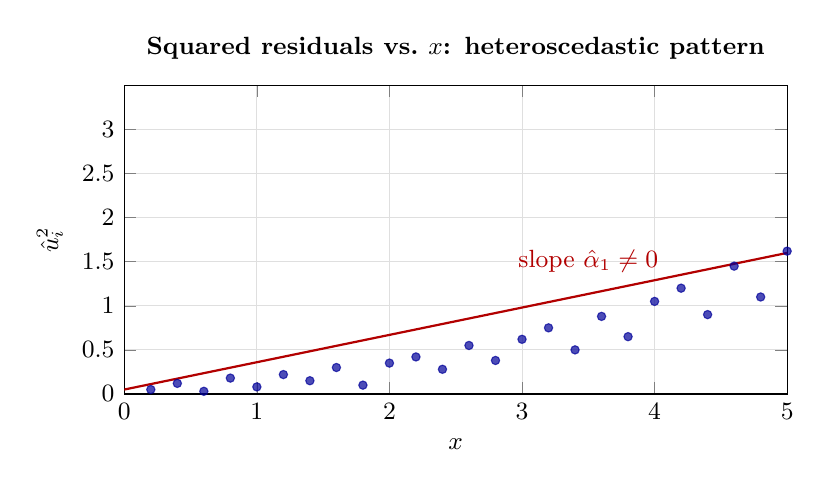
\begin{tikzpicture}
\begin{axis}[
  width=10cm, height=5.5cm,
  xlabel={$x$}, ylabel={$\hat u_i^2$},
  title={Squared residuals vs.\ $x$: heteroscedastic pattern},
  grid=both, grid style={line width=0.3pt, draw=gray!25},
  xmin=0, xmax=5, ymin=0, ymax=3.5,
  xtick={0,1,2,3,4,5}, ytick={0,0.5,1,1.5,2,2.5,3},
  tick label style={font=\small},
  title style={font=\small\bfseries},
  label style={font=\small}
]
\addplot[only marks, mark=*, mark size=1.5pt, blue!60!black, opacity=0.7]
  coordinates {
  (0.2,0.05)(0.4,0.12)(0.6,0.03)(0.8,0.18)(1.0,0.08)
  (1.2,0.22)(1.4,0.15)(1.6,0.30)(1.8,0.10)(2.0,0.35)
  (2.2,0.42)(2.4,0.28)(2.6,0.55)(2.8,0.38)(3.0,0.62)
  (3.2,0.75)(3.4,0.50)(3.6,0.88)(3.8,0.65)(4.0,1.05)
  (4.2,1.20)(4.4,0.90)(4.6,1.45)(4.8,1.10)(5.0,1.62)
  };
\addplot[thick, red!70!black, domain=0:5] {0.05 + 0.31*x};
\node[font=\small, red!70!black] at (axis cs:3.5,1.5) {slope $\hat\alpha_1 \neq 0$};
\end{axis}
\end{tikzpicture}
\end{center}

\begin{center}
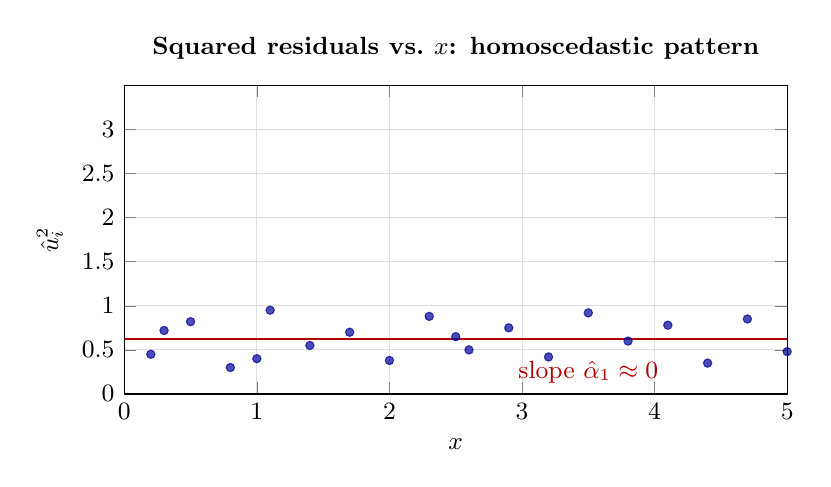
\begin{tikzpicture}
\begin{axis}[
  width=10cm, height=5.5cm,
  xlabel={$x$}, ylabel={$\hat u_i^2$},
  title={Squared residuals vs.\ $x$: homoscedastic pattern},
  grid=both, grid style={line width=0.3pt, draw=gray!25},
  xmin=0, xmax=5, ymin=0, ymax=3.5,
  xtick={0,1,2,3,4,5}, ytick={0,0.5,1,1.5,2,2.5,3},
  tick label style={font=\small},
  title style={font=\small\bfseries},
  label style={font=\small}
]
\addplot[only marks, mark=*, mark size=1.5pt, blue!60!black, opacity=0.7]
  coordinates {
  (0.2,0.45)(0.5,0.82)(0.8,0.30)(1.1,0.95)(1.4,0.55)
  (1.7,0.70)(2.0,0.38)(2.3,0.88)(2.6,0.50)(2.9,0.75)
  (3.2,0.42)(3.5,0.92)(3.8,0.60)(4.1,0.78)(4.4,0.35)
  (4.7,0.85)(5.0,0.48)(0.3,0.72)(1.0,0.40)(2.5,0.65)
  };
\addplot[thick, red!70!black, domain=0:5] {0.62};
\node[font=\small, red!70!black] at (axis cs:3.5,0.25) {slope $\hat\alpha_1 \approx 0$};
\end{axis}
\end{tikzpicture}
\end{center}

\subsection{Parametrization, Nuisance Parameters, and Composite Hypotheses}
\label{subsec:param_hyp}

We follow the Probabilist's notes of June~23, 2026.

\subsubsection*{When a hypothesis does not identify the measure}

A statistical model is a family of probability measures
$\{P_\theta : \theta \in \Theta\}$.
A hypothesis is a restriction on $\Theta$ — a subset $H \subseteq \Theta$.
The hypothesis determines not a single measure but a sub-family
$\{P_\theta : \theta \in H\}$.

\begin{definition}
A hypothesis $H$ is \textbf{simple} if it contains a single
parameter point, $H = \{\theta_0\}$, so that $P_\theta$ is uniquely
identified under $H$.  It is \textbf{composite} if $|H| > 1$.
\end{definition}

The key situation: the parameter space factors as
$\Theta = \Theta_1 \times \Theta_2$, and the hypothesis concerns
only one component:
\[
  H_0:\; \theta_1 = \theta_{1,0},
  \qquad\text{i.e.}\quad
  H_0 = \{\theta_{1,0}\} \times \Theta_2 \;\subseteq\; \Theta.
\]
This is a composite hypothesis whenever $|\Theta_2| > 1$.
The component $\theta_2$ is a \textbf{nuisance parameter}: it
enters the model and is estimated, but is not the target of the
test.  It remains free under both $H_0$ and $H_a$.

\begin{remark}
The alternative $H_a = (\Theta_1 \setminus \{\theta_{1,0}\}) \times
\Theta_2$ is also composite, for the same reason.  The nuisance
parameter $\theta_2$ is unspecified under both hypotheses.  This
is the generic situation in practice.
\end{remark}

\subsubsection*{Three cases}

The mutual structure of $H_0$ and $H_a$ in the parameter space
determines the complexity of the testing problem.

\textbf{Case~1: Both $H_0$ and $H_a$ are simple.}
Both hypotheses identify a single measure.  This requires the
model to be fully specified under each hypothesis — no free
parameters on either side.  This situation is essentially
theoretical; it is the setting of the Neyman--Pearson lemma,
where the most powerful test exists and is given by the
likelihood ratio.

\textbf{Case~2: $H_0$ is simple, $H_a$ is composite.}
The null is a single measure; the alternative is a family.
This requires $\Theta_2$ to be a singleton — the nuisance
parameter is known.  The structure of $H_a$ in the parameter
space matters for power, but the null distribution of any
test statistic is fully determined (since there is only one
null measure).  This case is rare in regression: it requires
knowing $\sigma^2$ (or all $\sigma_i^2$) under $H_0$.

\textbf{Case~3: Neither $H_0$ nor $H_a$ is simple.}
Both contain infinitely many measures.  This is the generic
case in regression.  Now the nuisance parameter $\theta_2$
is free on both sides, and its interaction with $\theta_1$
— the \emph{mutual location and structure} of $H_0$ and
$H_a$ in $\Theta$ — is the central difficulty.  The null
distribution of any test statistic depends on how $\theta_2$
is handled (estimated, profiled out, or otherwise eliminated).

\begin{remark}[the Probabilist's question]
When we have parameters $(\theta_1, \theta_2)$ and formulate
$H_0: \theta_1 = \theta_{1,0}$ with $\theta_2$ unspecified,
we are in Case~3: both $H_0 = \{\theta_{1,0}\} \times \Theta_2$
and $H_a = (\Theta_1 \setminus \{\theta_{1,0}\}) \times \Theta_2$
are composite.  So yes: having several parameters but testing
only one of them is generically Case~3.
\end{remark}

\subsubsection*{Application to regression: three layers of parametrization}

The regression model $y_i = \beta^\top x_i + u_i$ involves
parameters at three distinct levels.  At each level, the testing
problem is Case~3, but the nuisance space shrinks as we impose
more structure.

\subsubsection*{Layer~1: The regression coefficients $\beta$}

The most primitive parametrization of the model treats each error
variance as a free parameter:
\[
  \theta = (\beta,\, \sigma_1^2,\ldots,\sigma_n^2)
  \;\in\; \mR^p \times \mR_{>0}^n.
\]
A hypothesis about a single regression coefficient, say
$H_0: \beta_j = 0$, leaves all of $\beta_{-j}$ and all
$\sigma_i^2$ free.  The nuisance space is $\mR^{p-1} \times
\mR_{>0}^n$, which has dimension $p - 1 + n$ — it grows with
the sample size.  No finite-dimensional sufficient reduction exists,
and no standard test statistic has a tractable null distribution
without further restrictions.  The $t$-test for $\beta_j = 0$
only becomes available after imposing homoscedasticity (Layer~2
below).

\subsubsection*{Layer~2: The error variances $\sigma^2$}

Homoscedasticity replaces the $n$-dimensional nuisance
$(\sigma_1^2,\ldots,\sigma_n^2)$ with a single scalar $\sigma^2$:
\[
  \theta = (\beta,\, \sigma^2)
  \;\in\; \mR^p \times \mR_{>0}.
\]
The nuisance space is now finite-dimensional and does not grow
with $n$.  The OLS estimator $\hat\beta$ and the residual
variance $\hat\sigma^2$ are jointly sufficient; the $t$- and
$F$-statistics are pivotal under normality.  This is still
Case~3 (both $H_0: \beta_j = 0$ and $H_a$ are composite, since
$\sigma^2$ is free on both sides), but the nuisance is manageable.

Testing homoscedasticity itself — $H_0: \sigma_1^2 = \cdots =
\sigma_n^2$ — cannot be formulated within this layer, because the
constraint being tested is \emph{the defining assumption of the
layer}.  To test it, we need the richer parametrization of
Layer~1, restricted in a structured way.

\subsubsection*{Layer~3: The variance regressors $\alpha$}

The Breusch--Pagan test imposes a parametric form on the variances:
\[
  \sigma_i^2 = h(\alpha^\top z_i),
  \qquad
  \alpha = (\alpha_0,\alpha_1,\ldots,\alpha_q)^\top.
\]
This replaces the $n$-dimensional nuisance of Layer~1 with a
$(q+1)$-dimensional parameter $\alpha$, making the problem
tractable.  The full parameter is now
\[
  \theta = (\beta,\, \alpha)
  \;\in\; \mR^p \times \mR^{q+1}.
\]
The homoscedasticity null is
\[
  H_0:\; \alpha_1 = \cdots = \alpha_q = 0,
\]
which constrains $q$ components of $\alpha$ to zero while
leaving $\beta$ and $\alpha_0$ free.  Under $H_0$, the
nuisance is $(\beta, \alpha_0) \in \mR^p \times \mR$; under
$H_a$, it is $(\beta, \alpha) \in \mR^p \times \mR^{q+1}$.
Both are composite: Case~3.

The structure is now tractable, however.  The score (LM) test
evaluates the gradient of the log-likelihood with respect to the
$q$ constrained components $(\alpha_1,\ldots,\alpha_q)$ at the
restricted MLE (= OLS under $H_0$).  Under regularity conditions,
the LM statistic has a limiting $\chi^2_q$ distribution — with
$q$ degrees of freedom equal to the number of restrictions imposed
by $H_0$.

\begin{remark}[Degrees of freedom as a count of restrictions]
The $\chi^2_q$ in the BP test counts the number of \emph{scalar}
restrictions imposed by $H_0$, not the dimension of the nuisance
parameter or the full parameter space.  Each of $\alpha_1,\ldots,
\alpha_q$ is set to zero: that is $q$ restrictions, giving
$\chi^2_q$.  In simple regression with a single variance regressor
($q=1$), this is $\chi^2_1$.  In multiple regression with $k$
variance regressors ($q=k$), it is $\chi^2_k$.
\end{remark}

The three layers are summarised in Table~\ref{tab:layers}.

\begin{table}[ht]
\centering
\small
\begin{tabular}{llll}
\toprule
Layer & Parameter & Nuisance dimension & Testing problem \\
\midrule
1 ($\beta$ only) & $(\beta,\sigma_1^2,\ldots,\sigma_n^2)$ & $p-1+n$ (grows) & Intractable without structure \\
2 (homosc.)      & $(\beta,\sigma^2)$                     & $p$ (fixed)     & $t$/$F$ tests; pivot exact \\
3 (BP)           & $(\beta,\alpha_0,\alpha_1,\ldots,\alpha_q)$ & $p+1$ (fixed) & LM test; $\chi^2_q$ asymp. \\
\bottomrule
\end{tabular}
\caption{Three layers of parametrization in the BP regression model.
At each layer the testing problem is Case~3 (both $H_0$ and $H_a$
composite), but the nuisance space shrinks from $O(n)$ to a fixed
finite dimension, making standard inference feasible.}
\label{tab:layers}
\end{table}

%--------------------------------------------------------------------

\subsection{The Breusch--Pagan test: formal setup}

\textbf{Model.} Linear model with error variance
$\Var(u_i \mid x_i) = h(\alpha_0 + \alpha_1 x_i)$
for some function $h$.  The null hypothesis is
\[
  H_0: \alpha_1 = 0
  \qquad (\text{variance does not depend on }x).
\]
Under $H_0$, $\Var(u_i\mid x_i)=\sigma^2=h(\alpha_0)$: homoscedasticity.

\textbf{Test procedure.}
Since $u_i$ is unobservable, replace it by OLS residuals $\hat u_i$:
\begin{enumerate}[label=\arabic*.]
  \item Fit OLS to obtain residuals $\hat u_i$.
  \item Run the auxiliary OLS regression of $\hat u_i^2$ on $x_i$
    (and a constant).
  \item Compute $nR^2$ from this auxiliary regression.
  \item Under $H_0$: $nR^2 \xrightarrow{d} \chi^2_1$
    ($\chi^2_k$ for $k$ regressors).
  \item Reject $H_0$ at level $\alpha$ if $nR^2 > \chi^2_{1,\alpha}$.
\end{enumerate}

The statistic $nR^2$ is the LM statistic evaluated under $H_0$:
its form as $n$ times the $R^2$ of the auxiliary regression is a
consequence of applying the general LM principle to the normal
likelihood, where the score and Fisher information take a
particularly simple form.

\begin{remark}
The $\chi^2$ distribution is asymptotic. The original Breusch--Pagan
test assumed normality of $u$; the version due to Koenker (the
``studentised'' BP test) does not require normality and is more
robust in small samples.
\end{remark}

%--------------------------------------------------------------------

\subsection{Multivariate model setup and the nature of \texorpdfstring{$H_0$}{H0}}
\label{subsec:bp-setup}

We follow the Probabilist's notes of June~21, 2026.

\subsubsection*{The regression model}

The general linear regression model with $n$ observations and $p$
regressors is
\[
  \begin{cases}
    y_1 = \beta^\top x_1 + u_1 \\
    \quad\vdots \\
    y_n = \beta^\top x_n + u_n,
  \end{cases}
\]
where each regressor vector is a column:
\[
  \begin{cases}
    x_1 = (x_{11},\ldots,x_{1p})^\top \\
    \quad\vdots \\
    x_n = (x_{n1},\ldots,x_{np})^\top.
  \end{cases}
\]
The errors are independently normally distributed:
\[
  u_i \;\sim\; \mathrm{indep}\; \mathcal{N}(0,\,\sigma_i^2),
\]
so that in vector form
\[
  u = (u_1,\ldots,u_n)^\top
  \;\sim\;
  \mathcal{N}\!\bigl(0_n,\;\mathrm{diag}(\sigma_1^2,\ldots,\sigma_n^2)\bigr).
\]

\subsubsection*{Parametric variance structure}

The main modelling assumption of the BP test: each error variance
can be written as
\[
  \sigma_i^2 \;=\; h(\alpha^\top z_i),
\]
where $h(\cdot)$ is a twice-differentiable positive function,
$\alpha = (\alpha_0, \alpha_1, \ldots, \alpha_q)^\top$ is the
\emph{variance parameter vector}, and $z_i = (1, z_{i1}, \ldots,
z_{iq})^\top$ is an observable vector of \emph{variance regressors}
(often $z_i = x_i$, but not necessarily).

\subsubsection*{The null hypothesis and its character}

The homoscedasticity null is
\[
  H_0:\;\alpha_1 = \alpha_2 = \cdots = \alpha_q = 0,
\]
i.e.\ all slope components of $\alpha$ are zero.  Under $H_0$,
$\sigma_i^2 = h(\alpha_0) =: \sigma^2$ for all~$i$ — a constant.

\begin{remark}[The null is not a simple hypothesis]
The Probabilist observes: $H_0$ is \emph{not} of the form ``the parameter equals
a specific value.''  It is a \emph{structural restriction} on the
parameter vector: it sets $q$ components of $\alpha$ to zero while
leaving $\alpha_0$ (and all of $\beta$) unrestricted.  The restricted
parameter space is therefore a proper subspace of dimension strictly
less than the full parameter space — but it is not a single point.
Hence $H_0$ is a \textbf{composite} hypothesis, not a simple one.
This distinction matters: the LM (score) test statistic has a
$\chi^2_q$ limiting distribution under $H_0$ precisely because $q$
restrictions are imposed, and the $\chi^2$ degrees of freedom count
the number of restrictions, not the dimension of the parameter space.
\end{remark}

%--------------------------------------------------------------------

\subsection{Conditional distribution of \texorpdfstring{$u_i$}{u\_i} and the status of \texorpdfstring{$\sigma_i^2$}{sigma\_i\^{}2}}
\label{subsec:cond-normal}

We follow the Probabilist's notes of June~24, 2026.

\subsubsection*{Notation: intercept convention and indexation}

We clarify the indexation of regressors.
The coefficient vector $\beta$ and the regressor vector $x_i$ each
have $p+1$ components indexed from~$0$:
\[
  \beta = (\beta_0, \beta_1, \ldots, \beta_p)^\top,
  \qquad
  x_i = (x_{i0},\, x_{i1},\ldots,\, x_{ip})^\top,
  \qquad
  x_{i0} \equiv 1 \text{ (intercept).}
\]
Then $\beta^\top x_i = \beta_0 + \beta_1 x_{i1} + \cdots + \beta_p x_{ip}$.
Similarly, the variance regressors satisfy
\[
  z_i = (z_{i0}, z_{i1}, \ldots, z_{iq})^\top,
  \qquad z_{i0} \equiv 1,
\]
so $\alpha^\top z_i = \alpha_0 + \alpha_1 z_{i1} + \cdots + \alpha_q z_{iq}$.
The intercept component in each vector absorbs the constant term
and is \emph{not} a free parameter to be tested.

\begin{remark}[Consistency with earlier notation]
In the Multivariate model setup subsection (§\,\ref{subsec:bp-setup})
we wrote $x_i \in \mathbb{R}^p$.  With the intercept convention, the
dimension is $p+1$.  No conflict arises if we interpret $p$ there as
the total number of columns including the intercept column.  The present
subsection adopts the explicit $0$-indexed convention throughout.
\end{remark}

\subsubsection*{Random variances: the problem}

The Probabilist raised the following issue.  In the BP model,
$\sigma_i^2 = h(\alpha^\top z_i)$.
If $z_i$ is itself a random vector (e.g.\ the observed regressors
on the $i$-th unit), then $\sigma_i^2$ is a \emph{random variable},
not a fixed parameter.  Random variances are not parameters in the
classical sense, and the log-likelihood cannot be written in the
usual form.

This is a genuine tension, and it is resolved — not avoided — by
working with \emph{conditional} distributions.

\subsubsection*{Conditional probability as a random variable}

Fix observation $i$.  The conditional probability of the event
$\{u_i \in A\}$ given $Z_i$ is defined as
\[
  P\{u_i \in A \mid Z_i\}
  \;=\;
  \E\bigl[\mathbf{1}_{u_i \in A} \mid Z_i\bigr],
\]
which is a $[0,1]$-valued random variable — measurable with respect
to $\sigma(Z_i)$ — defined up to a $P$-null set.
Here $Z_i$ stands for either the random vector itself or its
generated $\sigma$-algebra; the two phrasings are equivalent.

\begin{remark}
This is conditioning with respect to a \emph{random variable},
not with respect to an event.  In particular,
$P\{u_i \in A \mid Z_i = z\}$ for a fixed value
$z \in \mathbb{R}^{q+1}$ requires care: the event $\{Z_i = z\}$
has probability zero when $Z_i$ is continuous, so the conditional
probability cannot be defined as a ratio.  The rigorous object is
the \emph{regular conditional distribution}, defined below.
\end{remark}

\subsubsection*{The kernel representation}

For $P$-almost every $\omega$, the map $A \mapsto P\{u_i \in A \mid Z_i\}(\omega)$
is a probability measure on $\mathbb{R}$.  Writing $z = Z_i(\omega)$,
we define the \textbf{conditional distribution kernel}
\[
  \mu_i(z,\, A) \;:=\; P\{u_i \in A \mid Z_i\}(\omega),
\]
so that $\mu_i\colon \mathbb{R}^{q+1} \times \mathcal{B}(\mathbb{R})
\to [0,1]$.  For every fixed $z \in \mathbb{R}^{q+1}$, the map
$A \mapsto \mu_i(z, A)$ is a probability measure on $\mathbb{R}$
(the distribution of $u_i$ given $Z_i = z$).  For every fixed
Borel set $A$, the map $z \mapsto \mu_i(z, A)$ is measurable.

\begin{remark}[Deterministic map from $\mathbb{R}^{q+1}$ to measures]
The Probabilist's key observation: what we actually need is not the full
random-measure object $\omega \mapsto \mu_i(Z_i(\omega), \cdot)$,
but the \emph{deterministic} function $z \mapsto \mu_i(z, \cdot)$.
This function maps each fixed vector $z \in \mathbb{R}^{q+1}$ to
a specific probability measure on $\mathbb{R}$.  The randomness of
$Z_i$ only matters when we integrate over it — which we do not need
for the likelihood computation, where $z_i$ are treated as fixed
design points.
\end{remark}

\subsubsection*{The BP distributional assumption}

Under the simplification of Breusch and Pagan, the conditional
distribution of each $u_i$ given $Z_i = z$ is normal with mean
zero and variance $h(\alpha^\top z)$:
\[
  \mu_i(z,\,\cdot\,) \;=\; \mathcal{N}\!\bigl(0,\; h(\alpha^\top z)\bigr).
\]
In the notation of the random-variable form:
\[
  u_i \mid Z_i \;\sim\; \mathcal{N}\!\bigl(0,\; h(\alpha^\top Z_i)\bigr).
\]
The full statement in the original Breusch--Pagan paper is stronger:
the entire error vector $u$ has a \emph{joint} Gaussian conditional
distribution given $Z = (z_1,\ldots,z_n)$:
\[
  u \mid Z \;\sim\;
  \mathcal{N}\!\Bigl(0_n,\;\operatorname{diag}\bigl(h(\alpha^\top z_i)\bigr)_{i=1}^n\Bigr).
\]
The diagonal covariance encodes both normality of each $u_i$ and
mutual independence of $u_1,\ldots,u_n$ given $Z$.

\begin{remark}[From conditional to ``unconditional'']
The Probabilist notes that writing the distribution of $u$ without conditioning
on $Z$ is informal: when $Z_i$ is a continuous random vector,
$P(Z_i = z_i) = 0$ for any fixed $z_i \in \mathbb{R}^{q+1}$, so
the conditional statement $u \mid Z_i = z_i$ cannot be interpreted
as ordinary conditional probability with respect to an event.  The
rigorous sense is exactly the kernel $\mu_i(z_i, \cdot)$ constructed
above.  For the likelihood this is harmless: the log-likelihood is
written as a function of the observed $z_i$ values, treating them as
deterministic inputs, which corresponds to the standard fixed-regressor
convention in regression analysis.
\end{remark}

\begin{remark}[Do we need random measures?]
The Probabilist's notes acknowledge a mild self-contradiction: the stated goal
was to avoid random measures, yet the conditional probability
$\omega \mapsto \mu_i(Z_i(\omega), \cdot)$ is precisely a
random measure.  The resolution is pragmatic: we invoke random
measures only to \emph{justify} the existence and measurability of
the kernel $\mu_i(z,\cdot)$ (this is the content of the regular
conditional distribution theorem), after which we work entirely with
the deterministic function $z \mapsto \mu_i(z, \cdot)$ and need
not refer to random measures again.
\end{remark}

% ---- continuation: the Probabilist--Boris dialogue, June 25, 2026 ----

\subsubsection*{The incidental parameters problem}

We follow the Probabilist's notes of June~25, 2026.

Returning to the free-variance model $u_i \sim \mathrm{indep}\,
\mathcal{N}(0, \sigma_i^2)$: the Probabilist notes that in this formulation
there is \emph{no way to estimate the $\sigma_i^2$ consistently}.
Each observation $u_i$ (equivalently, each residual $\hat u_i$) is
a single data point drawn from $\mathcal{N}(0, \sigma_i^2)$; a new
observation $u_{n+1}$ arrives with its own fresh $\sigma_{n+1}^2$
and tells us nothing about the previous variances.  The number of
free parameters grows with~$n$, so the MLE of $\sigma_i^2$ cannot
converge.

\begin{remark}[Incidental parameters]
This is the classical \emph{incidental parameters problem} (Neyman
and Scott, 1948).  The $\sigma_i^2$ are ``incidental'' parameters —
one per observation — as opposed to ``structural'' parameters such
as~$\beta$, which are shared across all observations.  The MLE of
incidental parameters is generally inconsistent and, crucially, its
inconsistency contaminates the MLE of the structural parameters too.
The BP parametrisation $\sigma_i^2 = h(\alpha^\top z_i)$ is
precisely the fix: it replaces $n$ incidental parameters with
$q + 1$ structural ones, restoring consistency.
\end{remark}

The Probabilist also notes the connection to Bayesian hierarchical models:
imposing $\sigma_i^2 = h(\alpha^\top z_i)$ with~$z_i$ i.i.d.\
is analogous to placing a parametric prior on the $\sigma_i^2$ and
treating the shared parameter~$\alpha$ as a hyperparameter.

\subsubsection*{Does $z_i = x_i$ imply homoscedasticity?}

Boris raised the following question.  The authors of the BP paper
remark that often $z_i = x_i$ is a natural choice.  If in addition
$x_i$ are i.i.d., then $\sigma_i^2 = h(\alpha^\top x_i)$ are
i.i.d.\ random variables.  Does this make the $u_i$ i.i.d., and
therefore homoscedastic?

\textbf{The Probabilist's answer: no.}  Homoscedasticity as defined in our
earlier chapters requires the conditional variance to be both
\emph{constant} and \emph{deterministic}:
\[
  \Var(u_i \mid x_i) \;=\; \sigma^2
  \quad \text{(the same fixed real number for all }i\text{).}
\]
Even if the random variables $\sigma_i^2 = h(\alpha^\top x_i)$ are
identically distributed — which they are when $x_i$ are i.i.d.\ —
they are still random, not constant.  Identity in distribution is
strictly weaker than equality as numbers.

\begin{remark}[Gradations of ``equal variance'']
The Probabilist identifies two intermediate statements between ``i.i.d.''\
and homoscedasticity:
\begin{enumerate}
\item \emph{Identically distributed:}
  $\sigma_1^2 \overset{d}{=} \sigma_2^2 \overset{d}{=} \cdots$
  (same law, but they may take different values on any given~$\omega$).
  Not homoscedasticity.
\item \emph{Pointwise equal:}
  $\sigma_1^2(\omega) = \sigma_2^2(\omega)$ for all $\omega \in \Omega$.
  This is a much stronger statement — it means the random variables
  are modifications of each other — but it is still not
  homoscedasticity, because the common value $\sigma^2(\omega)$ is
  still random and not a constant.
\end{enumerate}
The Probabilist notes that statement~(2) is hard to imagine in any realistic
model and is cited here only for conceptual completeness.
The upshot: randomness of $\sigma_i$ is not an obstacle to be
eliminated but a feature that \emph{defines} heteroscedasticity in
the random-regressor framework.
\end{remark}

\subsubsection*{Conditioning on $z$ versus conditioning on $x$}

The Probabilist raises a further subtlety.  Our definition of homoscedasticity
throughout these notes conditions on the regression regressors~$x_i$:
\[
  \Var(u_i \mid x_i) = \sigma^2.
\]
The BP test, however, parametrises variance through the auxiliary
vector~$z_i$, which may differ from~$x_i$.  The condition being
tested is therefore
\[
  \Var(u_i \mid z_i) = \sigma^2,
\]
a statement about a different conditioning sigma-algebra.  When
$z_i \neq x_i$ (e.g.\ $z_i$ contains functions of $x_i$ or
additional covariates), the BP test does not directly test our
earlier homoscedasticity definition.

The BP paper does not address this gap.  As the Probabilist puts it: it is
swept under the rug.  A careful treatment would require either
(a)~taking $z_i = x_i$ explicitly, in which case both definitions
coincide; or (b)~reformulating homoscedasticity relative to the
larger $\sigma$-algebra $\sigma(x_i, z_i)$.  We flag this as an
open point in our exposition.

\begin{remark}[Reference gap]
The Probabilist consulted the \emph{International Encyclopedia of
Statistics} (multi-author, $\sim$2016, over 1700 pages).  The
entry on heteroscedasticity did not provide a formal definition of
homoscedasticity.  This is symptomatic of a broader pattern in the
statistics literature: the term is used freely without a
measure-theoretic anchor.
\end{remark}

\subsubsection*{A note on the institutional gap between probability and statistics}

Boris observes: having studied statistics at three Canadian
universities (SFU, Western, UofT), he found that only UofT had
probability-specialist faculty and included measure-theoretic
probability as a standard component of the PhD curriculum.  At most
departments the typical PhD statistician completes their degree
without ever having taken a graduate-level probability course.
From this Boris draws the inference: expecting rigorously
probability-grounded arguments in mainstream statistics papers is
structurally unrealistic, because the institutional pipeline does
not produce researchers with those tools.

The observation extends to the disciplinary split Boris notes:
probability theory has penetrated quantitative finance far more
deeply than it has statistics itself.  Stochastic calculus, risk-neutral
pricing, and measure-theoretic foundations of martingale theory became
standard in financial mathematics from the 1970s onward, driven by
Black--Scholes and the Itô calculus.  In contrast, most working
statisticians operate with a toolkit grounded in Fisher, Neyman, and
Pearson — a framework that predates Kolmogorov's axiomatisation and
was never reformulated in its terms.

\begin{remark}[Claude's observation]
Boris's question — whether probability is penetrating more areas or
retreating — does not have a single answer.  The picture bifurcates.
On one side: machine learning and modern data science have
\emph{reduced} the role of measure-theoretic probability, replacing
it with finite-sample concentration inequalities and computational
heuristics.  A practitioner training neural networks operates entirely
outside Kolmogorov's framework.  On the other side: areas such as
nonparametric Bayes (Gaussian processes, Dirichlet processes), causal
inference under interference, and robust statistics have
\emph{increased} their reliance on advanced probability.

The finance example is worth unpacking.  Measure theory entered
finance not because financial economists sought mathematical rigour
for its own sake, but because the problems demanded it: pricing
derivatives required integrating over continuous paths, and the only
tools for that were stochastic integration and change-of-measure
arguments.  The tool followed the problem.  Statistics, by contrast,
has problems (conditional independence, exchangeability, nonparametric
priors) that equally demand measure theory — but the discipline's
culture and training infrastructure have not converged to the same
conclusion.

Whether this changes depends less on abstract intellectual trends
than on institutional incentives: hiring committees, qualifying
exam syllabi, and journal referee expectations.  Boris's experience
across three universities is a precise diagnostic of where those
incentives currently sit.
\end{remark}

%--------------------------------------------------------------------

\subsection{The Koenker (1981) modification: non-conditional parametrization}
\label{subsec:koenker}

We follow Boris's notes of June~27, 2026 (note~52).

\subsubsection*{A paper the Probabilist brought}

The Probabilist brought the paper: Roger Koenker, ``A note on studentizing a test
for heteroscedasticity,'' \textit{Journal of Econometrics}~17 (1981),
107--112.  The paper modifies the assumptions of the BP test and
proposes a small change to the test statistic.

\subsubsection*{The product parametrization}

Koenker works with the following model, which the Probabilist notes avoids
conditional distributions entirely:
\begin{align}
  y_i &= x_i\beta + u_i, \tag{1.1} \\[3pt]
  u_i &= \sigma_i\varepsilon_i, \tag{1.2} \\[3pt]
  \sigma_i &= 1 + h(z_i\gamma), \tag{1.3}
\end{align}
where $x_i$ and $z_i$ are row vectors of known constants (fixed
regressors), $h$ is a smooth positive function with $h(0) = 0$, and
$\varepsilon_i$ are i.i.d.\ with mean~$0$, variance~$\sigma^2$, and
finite fourth moment.  The null hypothesis is $H_0: \gamma = 0$, under
which $\sigma_i = 1$ and $u_i = \sigma\varepsilon_i$ is homoscedastic.

\begin{remark}[Product model vs.\ conditional normal]
BP's original model specifies a conditional normal distribution for
$u_i$ given~$z_i$: $u_i \mid z_i \sim \mathcal{N}(0, h(\alpha^\top
z_i))$.  Koenker's product model (1.2) makes no normality assumption
on~$\varepsilon_i$; the distribution is an unspecified $F$ with finite
fourth moment.  The conditional distribution of~$u_i$ given $z_i$ in
Koenker's model is a scaled copy of~$F$, not necessarily Gaussian.
Note also that (1.3) parametrises the \emph{standard deviation}
$\sigma_i$, not the variance: $\sigma_i^2 = (1 + h(z_i\gamma))^2
\approx 1 + 2h(z_i\gamma)$ near $\gamma = 0$.
\end{remark}

\subsubsection*{The test statistic and the kurtosis problem}

BP base their test on the OLS residuals
$\hat{u} = [I - X(X'X)^{-1}X']u$,
the variance estimate $\hat{\sigma}^2 = \hat{u}'\hat{u}/n$,
and the centred squared residuals $\hat{w}_i = \hat{u}_i^2 -
\hat{\sigma}^2$.  The BP test statistic is
\[
  \hat\xi \;=\; \tfrac{1}{2}\hat{w}'Z(Z'Z)^{-1}Z'\hat{w}\,/\,\hat\sigma^4.
\]
Koenker's theorem shows that, without the Gaussian assumption on
$\varepsilon$, the rescaled statistic $\xi^* = \hat\xi/\lambda$
converges in distribution to a non-central $\chi^2_p(\eta)$, where
$\lambda = \phi/(2\sigma^4)$ and $\phi = \Var(\varepsilon^2)$.
Under Gaussian $\varepsilon$, $\phi = 2\sigma^4$ so $\lambda = 1$
and the size is correct.  Under non-Gaussian $\varepsilon$,
$\lambda \neq 1$ and the BP test has \textbf{asymptotically incorrect
size}: the nominal $\alpha$ level is not achieved.

The fix Koenker proposes: replace $2\hat\sigma^4$ in the denominator
by $\hat\phi = (1/n)\sum_i \hat{w}_i^2$.  Since $\hat\phi \to \phi$
in probability, the modified statistic $\hat\alpha'Z'Z\hat\alpha /
\hat\phi$ has the correct limiting $\chi^2_p$ distribution under $H_0$
without Gaussianity.  Koenker notes that this modified statistic
equals $nR^2$, where $R^2$ is the \emph{uncentred} coefficient of
determination in the auxiliary regression of $\hat{w}$ on~$Z$.

\subsubsection*{Boris's observation: where are the type~I and II error statements?}

Boris notes a gap that applies to both the original BP paper and
Koenker's note: neither paper contains an explicit statement about
type~I or type~II error probabilities of the test.  What both papers
provide is an asymptotic distribution result for the test
\emph{statistic} under $H_0$ (and, in Koenker, under contiguous
alternatives).

The Probabilist confirms: the asymptotic distribution of the test statistic is
what is proved.  Mention of power appears near the end of Koenker's
paper, but without exact statements or computations.

\begin{remark}[Distribution of the statistic is not the same as error probability control]
Knowing that $\hat\xi \xrightarrow{d} \chi^2_p$ under $H_0$ is a
necessary condition for the test to have asymptotically correct size,
but it is not sufficient on its own.  For the rejection rule
``reject if $\hat\xi > \chi^2_p(1-\alpha)$'' to have limiting type~I
error $\alpha$, one additionally needs the convergence to be
sufficiently uniform over the null (or at least to hold for all
$\theta \in H_0$) and needs the quantile of the limit distribution to
be a continuity point.  These are standard but non-trivial conditions
that the econometrics literature commonly treats as understood.
Boris's observation is that they are, strictly speaking, not stated.
The gap the Probabilist and Boris identify here connects directly to the
foundational questions in note~53.
\end{remark}

%--------------------------------------------------------------------

\subsection{Asymptotic test behaviour and the notion of consistency}
\label{subsec:asymp-test}

We follow Boris's notes of June~27, 2026 (note~53).

\subsubsection*{What ``the test'' actually is}

When we casually say ``a test,'' we sweep under the rug that in fact
it is a \emph{parametrized family} of tests.  For the tests we
encounter in practice, the family is parametrized by at least two
quantities: the significance level~$\alpha$ and the sample size~$n$.
A test at level~$\alpha$ for sample size~$n$ is a measurable function
$\phi_{n,\alpha}\colon \mathcal{X}^n \to \{0,1\}$ (reject or not),
so what we call ``the BP test'' is really the collection
$\{\phi_{n,\alpha} : n \geq 1,\, \alpha \in (0,1)\}$.

\subsubsection*{Type~I and II error probabilities}

For a fixed test $\phi_{n,\alpha}$ and a fixed parameter
value~$\theta$:
\begin{align*}
  \alpha_n(\theta) &:= P_\theta(\phi_{n,\alpha} = 1),
  \quad \theta \in H_0, \\
  \beta_n(\theta) &:= P_\theta(\phi_{n,\alpha} = 0),
  \quad \theta \in H_a.
\end{align*}
When both hypotheses are simple (single measures), $\alpha_n$ and
$\beta_n$ are single numbers.  When $H_0$ or $H_a$ is composite,
$\alpha_n(\theta)$ and $\beta_n(\theta)$ depend on the specific
$\theta$, and there is no single ``the $\alpha$'' or ``the $\beta$'':
they are functions on the respective hypothesis sets.

In practice one controls the \emph{supremum}:
\[
  \sup_{\theta \in H_0} \alpha_n(\theta) \;\leq\; \tilde\alpha_n
  \qquad\text{and}\qquad
  \sup_{\theta \in H_a} \beta_n(\theta) \;\leq\; \tilde\beta_n.
\]
These upper bounds $\tilde\alpha_n$ and $\tilde\beta_n$ are the
quantities one can actually quote as guarantees.

\subsubsection*{Consistency of a sequence of tests}

The asymptotic analog of the above: choose a sequence of tests
$\phi_{n,\alpha_n}$ with the goal that both error bounds converge to
zero:
\[
  (\tilde\alpha_n,\, \tilde\beta_n) \;\to\; (0, 0)
  \quad\text{as } n \to \infty.
\]
A sequence of tests achieving this is called \textbf{consistent}.
The Probabilist notes that this is how consistency of a test should be
understood in the composite-hypothesis setting: not convergence of
a single number, but convergence of a pair of uniform bounds.

\begin{remark}[Why $\alpha_n$ may need to depend on $n$]
The Probabilist cites a source in which Fisher argued it is unreasonable to fix
the same $\alpha$ level for all sample sizes.  The intuition: at very
large $n$, one can afford a smaller $\alpha$ (the test has more power
for any fixed alternative), so insisting on $\alpha = 0.05$ for
$n = 10^6$ may be wasteful or even misleading.  Allowing $\alpha_n
\to 0$ as $n \to \infty$ — while ensuring $\beta_n \to 0$ as well —
is a more honest calibration.  The pair $(\alpha_n, n)$ replaces the
single parameter $\alpha$ as the fundamental specification.
\end{remark}

\subsubsection*{The asymmetry of $H_0$ and $H_a$}

The Probabilist and Boris discuss why the standard framework treats $\alpha$ and
$\beta$ asymmetrically.  The standard undergraduate procedure is:
(1)~choose the $\alpha$-level parameter of the test (implemented
through a threshold on the statistic); (2)~$\beta$ then follows from
the sample size and the specific alternative — it is not chosen.  In
general, for a compound $H_a$, there is no single $\beta$ to choose:
it is a function of $\theta \in H_a$.

Boris traces this asymmetry to Fisher.  The conceptual origin: $H_0$
is the \emph{status quo} — a position held for years — while $H_a$ is
a \emph{challenger}.  We give the challenger a lower chance of
survival by requiring strong evidence to reject $H_0$.  This
framing predates Kolmogorov's 1933 axiomatisation; Fisher lived until
1962 and could in principle have encountered measure-theoretic
probability, but his framework was never reformulated in those terms.
The Neyman--Pearson elaboration formalised $\beta$ as a second
parameter, but the underlying asymmetry persists.

\begin{remark}[Structural reason $H_0$ is more often simple]
Boris observes: historically $H_0$ is more often a simple
hypothesis than $H_a$.  This is not arbitrary.  A natural $H_0$
is often a specific structural claim — independence, equality of
means, zero coefficient — which pins down the parameter exactly
(up to nuisance, which is then either known or eliminated by a pivot).
The alternative, being the negation, is typically composite: ``not
independent,'' ``unequal means,'' ``non-zero coefficient.''
Because $H_0$ is frequently simple, the literature on $\alpha$-level
control is richer and more explicit, while power analysis ($\beta$)
requires specifying a point in $H_a$ and is treated as a secondary,
design-stage consideration.
\end{remark}

%--------------------------------------------------------------------

\subsection{BP as a semi-parametric test: the difficulty of error bounds}
\label{subsec:semipar}

We follow Boris's notes of June~29, 2026 (note~54).

\subsubsection*{Classification vs.\ hypothesis testing: why consistency is harder here}

The Probabilist notes that $\alpha$ and $\beta$ recall binary classification problems.
The analogy is instructive precisely because it breaks down at a key
point.

In a binary classification problem one typically has an \emph{overall}
distribution on the sample space: $P = \pi P_0 + (1-\pi)P_1$, where
$\pi$ is the base rate (prior probability of class~1).  Given this, one
can define an overall misclassification rate — a single number combining
the frequency of~$0$s and~$1$s — and minimise it.  Consistency of a
classifier can be formulated as convergence of that rate to its Bayes
minimum.

In hypothesis testing there is no such overall measure.  The sample
comes from \emph{either} the $H_0$-family of measures \emph{or} the
$H_a$-family — not from a mixture.  No $\pi$ is given, and in the
frequentist framework none is sought.  Type~I and type~II errors are
therefore irreducibly separate quantities, each defined with respect to
a different family of measures.  This is why consistency of a test
sequence cannot be defined as convergence of a single number; the
$(\tilde\alpha_n, \tilde\beta_n) \to (0,0)$ formulation from
§\,\ref{subsec:asymp-test} is the correct two-dimensional substitute.

\subsubsection*{Why worst-case error bounds are hard for the BP test}

The Probabilist characterises the BP test as \emph{semi-parametric}: the model
specifies a parametric form for the conditional distribution of $Y$
given $(X,Z)$, but leaves the marginal distribution of $(X,Z)$
entirely unspecified.  In the fixed-regressor convention of Koenker's
paper, $x_i$ and $z_i$ are treated as known constants, so the question
of the distribution of~$X$ does not arise.  But when $X$ and $Z$ are
genuinely random, their joint distribution becomes an
infinite-dimensional nuisance parameter.

\begin{remark}[Why this matters for $\alpha$ and $\beta$]
In the fixed-regressor framework, the type~I error of the BP test is
controlled asymptotically by the $\chi^2_q$ limit: the design
conditions (A.1) of Koenker's paper ensure this uniformly over the
finite-dimensional nuisance $(\beta,\alpha_0)$.  The sup over all
possible fixed design sequences satisfying (A.1) is bounded.

In the random-regressor framework, the sup over all joint distributions
of $(X,Z)$ is a much larger object.  Without restricting that
distribution (e.g.\ to satisfy moment conditions or tail bounds), one
cannot bound $\tilde\alpha_n$ uniformly.  This is the semi-parametric
difficulty Boris identifies: the worst-case $\alpha$ and $\beta$ are
not well-defined without specifying a class of distributions for~$X$.
The BP paper and Koenker's note sidestep this by treating regressors as
fixed — a convention that handles the problem by assumption rather than
proof.
\end{remark}

%--------------------------------------------------------------------

\subsection{Return to the model: test statistic construction and the p-value gap}
\label{subsec:back-to-test}

We follow Boris's notes of June~29 -- July~1, 2026 (note~55).

\subsubsection*{The model in Koenker's formulation}

We restate the model cleanly.  There exist deterministic unknown
parameter vectors
\[
  \beta = (\beta_0, \beta_1, \ldots, \beta_p)^\top,
  \qquad
  \alpha = (\alpha_0, \alpha_1, \ldots, \alpha_q)^\top,
\]
and random variables $(Y_i, X_i, Z_i)$, all observed, related by
\begin{align*}
  Y_i &= \beta^\top X_i + U_i, \\
  U_i &= \sigma_i\,\varepsilon_i, \qquad \varepsilon_i \;\text{i.i.d.},
  \quad \E[\varepsilon_i]=0,\quad \Var(\varepsilon_i)=\sigma^2, \\
  \sigma_i^2 &= h(\alpha^\top Z_i).
\end{align*}
The random variables $U_i$, $\sigma_i$, and $\varepsilon_i$ are
\emph{not} observed.  The parameters $\alpha$ and $\beta$ are
deterministic and unknown.  No relationship between $X_i$ and $Z_i$ is
assumed; they may coincide or be entirely separate.

\subsubsection*{Homoscedasticity and the null hypothesis}

Homoscedasticity requires two things of $\sigma_i$:
\begin{enumerate}
\item \textbf{Non-randomness:} $\sigma_i$ is a constant, not a random
  variable (it does not vary with the draw $\omega$).
\item \textbf{Constancy:} $\sigma_i$ is the same value for all $i$
  (follows from non-randomness if the parametric form $h(\alpha^\top
  Z_i)$ is used, since $h(\alpha^\top z)$ is deterministic when $z$ is
  a fixed vector and $\alpha$ is deterministic).
\end{enumerate}
In terms of the parameter $\alpha$, these conditions are equivalent to
\[
  \alpha \;=\; (\alpha_0, 0, \ldots, 0)^\top,
\]
i.e.\ the null hypothesis is
\[
  H_0:\; \alpha_1 = \alpha_2 = \cdots = \alpha_q = 0.
\]
Note that $\beta$ is unconstrained under $H_0$: we test the variance
structure, not the mean.  Also note that $\alpha_0$ is free under $H_0$
— it determines the common variance $\sigma^2 = h(\alpha_0)$.

\begin{remark}[Equivalence caveat]
Boris notes the equivalence between ``$\sigma_i$ constant'' and
``$\alpha_1 = \cdots = \alpha_q = 0$'' is not entirely obvious for
general $h$ and general $Z_i$.  For example, if $Z_i$ always lies in
a subspace where $h(\alpha^\top z) = h(\alpha_0)$, the slope
components of $\alpha$ are irrelevant even when non-zero.  For the
generic case — $Z_i$ spanning $\mathbb{R}^{q+1}$ in the sense of
condition (A.1) of Koenker — the equivalence holds.
\end{remark}

\subsubsection*{Construction of the test statistic}

The test proceeds in two stages.

\textbf{Stage~1: OLS residuals.}  Estimate $\beta$ by OLS on the
$(Y_i, X_i)$ pairs:
\[
  \hat\beta = (X^\top X)^{-1}X^\top Y,
  \qquad
  \hat U_i = Y_i - X_i^\top\hat\beta.
\]
Note that $\hat\beta$ itself is discarded after this step; only the
residuals $\hat U_i$ are used further.

\textbf{Stage~2: Auxiliary regression.}  Compute the pooled variance
estimate
\[
  \hat\sigma^2 \;=\; \frac{1}{n}\sum_{i=1}^n \hat U_i^2,
\]
and the normalised squared residuals
\[
  g_i \;=\; \frac{\hat U_i^2}{\hat\sigma^2}.
\]
The BP paper uses the notation $g_i$ (the Probabilist notes it is not an
especially descriptive name).  Observe that $\frac{1}{n}\sum_i g_i = 1$
by construction, so the $g_i$ are centred at~$1$.  Under $H_0$ and for
large $n$, $g_i \approx \varepsilon_i^2/\sigma^2$, which has mean~$1$
and is uncorrelated with $Z_i$.

Run the auxiliary OLS regression of $g_i$ onto $Z_i$:
\[
  g_i = Z_i^\top \hat\gamma + \text{residual}.
\]
The test statistic is \emph{half the explained sum of squares} of this
regression:
\[
  T_n \;=\; \tfrac{1}{2}\,\widehat{\mathrm{ESS}},
  \qquad
  \widehat{\mathrm{ESS}} = \hat\gamma^\top (Z^\top Z)\,\hat\gamma.
\]
Under $H_0$ and the Gaussian assumption, $T_n \xrightarrow{d} \chi^2_q$.

\begin{remark}[Degrees of freedom: $\chi^2_q$ not $\chi^2_{q-1}$]
Boris's note states the limit is $\chi^2_{q-1}$. This appears to be a
slip in counting.  The null imposes $q$ constraints
($\alpha_1 = \cdots = \alpha_q = 0$), so the LM statistic has $q$
degrees of freedom.  The vector $Z_i$ has $q+1$ components (including
the intercept $z_{i0} \equiv 1$), but the intercept column in the
auxiliary regression absorbs $\alpha_0$, which is \emph{not}
constrained — leaving exactly $q$ free directions being tested.
Koenker's theorem confirms: the limit distribution is $\chi^2_p$ in his
notation, where $p$ is the dimension of $\gamma$ (the slope part of
$\alpha$) — i.e.\ $q$ in ours.
\end{remark}

\subsubsection*{From the distribution of $T_n$ to a p-value: the remaining gap}

Boris adds (July~1, 2026): even for $\alpha$-level purposes, proving
$T_n \xrightarrow{d} \chi^2_q$ under $H_0$ is not sufficient on its
own.  Two additional steps are required.

\textbf{Step~A: Connecting the statistic to $\alpha$.}  The rejection
rule is ``reject $H_0$ if $T_n > c_{q,1-\alpha}$,'' where
$c_{q,1-\alpha}$ is the $(1-\alpha)$-quantile of $\chi^2_q$.  The
convergence $T_n \xrightarrow{d} \chi^2_q$ implies
\[
  P_{H_0}(T_n > c_{q,1-\alpha}) \;\to\; \alpha
  \quad \text{as } n \to \infty,
\]
provided $c_{q,1-\alpha}$ is a continuity point of the $\chi^2_q$
distribution (it is) and the convergence holds uniformly enough over
$H_0$.  This step is implicit in both the BP paper and Koenker's note
— it is treated as ``obvious from the convergence in distribution.''
Boris's point is that it is not trivial and is not explicitly stated.

\textbf{Step~B: The p-value.}  Boris notes that the p-value
$p_n = P(\chi^2_q \geq T_n^{\mathrm{obs}})$ is in principle
well-defined here because the limiting distribution is free of all
nuisance parameters ($\beta$ and $\alpha_0$ drop out of the limit).
This is a non-trivial property — it is the Wilks phenomenon for LM
tests — and it holds because the score evaluated at the restricted MLE
is asymptotically normal with covariance that does not depend on the
nuisance.

However, Boris's broader point stands: for more complicated hypothesis
structures (non-standard boundary cases, non-smooth parametrizations,
or non-interior null points), the p-value may fail to exist in the
usual sense, since there is no single scalar sufficient to rank
evidence against $H_0$.  The BP test happens to be in the favourable
regime — one-sided in each component of $\alpha$ aggregated into a
single LM quadratic form — but this should be stated, not assumed.

%--------------------------------------------------------------------

\subsection{Why the LM statistic is \texorpdfstring{$\chi^2$}{chi-squared}: centration and nuisance}
\label{subsec:chisq-centration}

We follow Boris's notes of July~2, 2026 (note~56).

\subsubsection*{Boris's question}

The standard argument that a score statistic is asymptotically $\chi^2_q$
under $H_0$ runs as follows.

\begin{enumerate}
\item \textbf{Centration.}  The score identity states that under the
  true measure $P_\theta$,
  \[
    E_\theta\!\left[\frac{\partial}{\partial\theta}\log p(X;\theta)\right] = 0.
  \]
  So the score is centered at zero under the native measure.

\item \textbf{CLT.}  With i.i.d.\ observations, the sum of individual
  scores obeys the CLT, and
  \[
    \frac{1}{\sqrt{n}}\sum_{t=1}^n \frac{\partial}{\partial\theta}\log p(x_t;\theta)
    \;\xrightarrow{d}\; \mathcal{N}(0,\,\mathcal{J}(\theta)).
  \]

\item \textbf{$\chi^2$.}  A centered normal divided by its standard
  deviation, squared, is $\chi^2_1$; the $q$-dimensional version gives
  $\chi^2_q$.
\end{enumerate}

Boris's worry: in the BP setting the measure is not fully specified
under $H_0$ — the nuisance parameters $(\beta, \alpha_0)$ are free.
So ``the native measure'' does not exist as a single $P_{\theta_0}$.
The score evaluated at the restricted MLE
$\hat\theta = (\hat\beta, \hat\alpha_0, 0)$ uses estimated nuisance
parameters, not the true ones.  Does centration survive?  And if the
score is not centered, the CLT produces a non-zero mean, the sum of
squares drifts positive, and the test over-rejects — no $\chi^2$.

\subsubsection*{Answer: centration holds pointwise, substitution error is negligible}

\textbf{Step 1: The score identity is pointwise in $\theta$.}
For each fixed $\theta_0 = (\beta_0, \alpha_{0,0}, 0) \in H_0$,
\[
  E_{\theta_0}\!\left[\frac{\partial}{\partial\alpha_j}\log p(x_t;\theta_0)\right] = 0,
  \qquad j = 1,\ldots,q.
\]
This holds by the usual differentiation-under-the-integral argument
and requires no knowledge of the nuisance values — only that $\theta_0$
is the true parameter.  Centration is a property of the score at the
\emph{true} $\theta$, not at an estimated one.

The difficulty Boris identifies is genuine: we cannot evaluate
$d_{\alpha_j}(\theta_0)$ because $\theta_0$ is unknown.  Instead we
substitute $\hat\theta$ (the constrained MLE under $H_0$), obtaining
$\hat d_{\alpha_j} = d_{\alpha_j}(\hat\theta)$.  Decompose:
\[
  \hat d_{\alpha_j}
  \;=\;
  \underbrace{d_{\alpha_j}(\theta_0)}_{\text{centered, mean 0}}
  \;+\;
  \underbrace{\bigl[d_{\alpha_j}(\hat\theta) - d_{\alpha_j}(\theta_0)\bigr]}_{\text{estimation error}}.
\]
The first term is centered.  The second is the price of using estimated
nuisance.

\textbf{Step 2: Block-diagonal structure kills the estimation error.}
The Fisher information matrix $\mathcal{J}$ is block-diagonal between
$(\beta, \alpha_0)$ and $(\alpha_1,\ldots,\alpha_q)$:
\[
  \mathcal{J}_{\alpha_j,\beta} = 0,
  \qquad
  \mathcal{J}_{\alpha_j,\alpha_0} = 0,
\]
as computed in our earlier example (the cross-derivative contains
$E[u_t] = 0$).  This means the constrained MLE satisfies
\[
  \sqrt{n}(\hat\beta - \beta_0) = O_p(1), \quad
  \sqrt{n}(\hat\alpha_0 - \alpha_{0,0}) = O_p(1),
\]
and the first-order Taylor expansion of the estimation error gives:
\[
  d_{\alpha_j}(\hat\theta) - d_{\alpha_j}(\theta_0)
  = \frac{\partial^2 l}{\partial\alpha_j\,\partial\beta}(\hat\beta-\beta_0)
  + \frac{\partial^2 l}{\partial\alpha_j\,\partial\alpha_0}(\hat\alpha_0-\alpha_{0,0})
  + o_p(\sqrt{n}).
\]
By the block-diagonal structure, the expected values of both
cross-second-derivative terms are zero.  After normalising by
$\sqrt{n}$, the estimation error is $o_p(1)$.  The centered term
$d_{\alpha_j}(\theta_0)/\sqrt{n}$ dominates, CLT applies, and the
$\chi^2$ limit goes through.

This is why BP do not simply cite the ``general score result'': the
general theorem assumes a fully specified measure.  BP need to carry
out the estimation-error accounting explicitly.

\subsubsection*{The Probabilist's three steps in the BP proof}

The Probabilist identifies the BP proof as three distinct steps.

\textbf{Step~1: Simplify the general LM statistic for block-diagonal $\mathcal{J}$.}
The full LM is $d'\mathcal{J}^{-1}d$.  Block-diagonal structure reduces
this to
\[
  \text{LM} = \hat d_\alpha' \hat{\mathcal{J}}_{\alpha\alpha}^{-1} \hat d_\alpha,
\]
where $\hat d_\alpha$ is the score in the $\alpha$-directions only,
evaluated at $\hat\theta$.  The nuisance block $(\beta, \alpha_0)$
drops out because $\hat d_\beta = \hat d_{\alpha_0} = 0$ at the
constrained MLE by the first-order conditions.

\textbf{Step~2: Evaluate the simplified statistic.}
Substituting the BP model and computing $\hat d_\alpha$ and
$\hat{\mathcal{J}}_{\alpha\alpha}$ explicitly (with $h'$ terms
cancelling), the LM statistic equals $\frac{1}{2}\,\widehat{\mathrm{ESS}}$
from the auxiliary regression of $g_t = \hat u_t^2/\hat\sigma^2$ on
$z_t$.  This is BP's Theorem.

\textbf{Step~3: Apply Amemiya's CLT for regression coefficients.}
Let $\hat\delta$ be the OLS coefficients in the auxiliary regression
of $g_t$ on $z_t$, and $S = \hat\delta'(Z'Z)\hat\delta$ the explained
sum of squares.  Amemiya (1977) shows that under $H_0$:
\[
  \sqrt{n}(\hat\delta - 0) \;\xrightarrow{d}\; \mathcal{N}(0,\;2\sigma^4 D^{-1}),
  \qquad D = \lim n^{-1}Z'Z.
\]
The coefficient $\hat\delta$ is asymptotically centred at zero because
$g_t$ is asymptotically uncorrelated with $z_t$ under $H_0$ — this is
the centration argument resolved: it is not the score itself that is
shown to be centered, but the auxiliary regression coefficient.  From
this CLT it follows that $(2\hat\sigma^4)^{-1}S \xrightarrow{d}
\chi^2_{p-1}$, which equals $\chi^2_q$ in our notation.

\begin{remark}[Why asymptotic centration works]
Boris conjectured that ``maybe there will be some asymptotic
centration.''  This is exactly right, but the route is indirect.
Under $H_0$, $g_t = \hat u_t^2/\hat\sigma^2 \approx
\varepsilon_t^2/\sigma^2$, which has mean~$1$ and is independent of
$z_t$ (since $\varepsilon_t$ are i.i.d.\ and $z_t$ are fixed design
points).  The auxiliary regression of $g_t$ on $z_t$ therefore has
true slope zero — this is the centration.  It is asymptotic because
it uses $\hat u_t$ rather than $u_t$, and the approximation
$\hat u_t \approx u_t$ is valid only for large $n$.
\end{remark}

\begin{remark}[Why BP do not invoke the general score theorem]
The general theorem states: if $T_n = n^{-1/2}\sum_t \partial\log p_t/
\partial\gamma \xrightarrow{d} \mathcal{N}(0,\mathcal{J})$ under $H_0$
(with $\gamma$ the tested parameter), then $\mathcal{J}^{-1/2}T_n$
has components that are asymptotically i.i.d.\ $\mathcal{N}(0,1)$, and
$\|{\mathcal{J}^{-1/2}T_n}\|^2 \xrightarrow{d} \chi^2_q$.  The theorem
requires that $\mathcal{J}$ and $T_n$ be evaluated at the \emph{true}
parameter.  With unknown nuisance, one must show that substituting
$\hat\theta$ for $\theta_0$ does not change the limit — and this is
precisely what Steps~1--3 above establish.  The general theorem
provides the framework; BP's three steps provide the model-specific
verification.
\end{remark}

%--------------------------------------------------------------------

\end{document}
